\documentclass[12pt,a4paper,oneside]{article}
\usepackage[T1]{fontenc}
\usepackage[utf8]{inputenc}
\usepackage[english,italian]{babel}
\usepackage{amsmath}
\usepackage{amsthm}
\usepackage{marvosym}
\usepackage{mathtools}
\usepackage[left=2cm,right=2cm,top=2cm,bottom=2cm]{geometry}       		
\usepackage{graphicx}		
\usepackage{subfig}		
\usepackage{amssymb}
\usepackage{braket}
\usepackage{mathtools}
\usepackage[usenames,dvipsnames]{color}   
\usepackage{hyperref}
\usepackage{caption}
\usepackage{listings} 
\usepackage[usenames,dvipsnames]{color}   
\lstset{ 
  language=R,                     % the language of the code
  basicstyle=\ttfamily, % the size of the fonts that are used for the code
  numbers=left,                   % where to put the line-numbers
  numberstyle=\color{Blue},  % the style that is used for the line-numbers
  stepnumber=1,                   % the step between two line-numbers. If it is 1, each line
                                  % will be numbered
  numbersep=5pt,                  % how far the line-numbers are from the code
  backgroundcolor=\color{white},  % choose the background color. You must add \usepackage{color}
  showspaces=false,               % show spaces adding particular underscores
  showstringspaces=false,         % underline spaces within strings
  showtabs=false,                 % show tabs within strings adding particular underscores
  frame=single,                   % adds a frame around the code
  rulecolor=\color{black},        % if not set, the frame-color may be changed on line-breaks within not-black text (e.g. commens (green here))
  tabsize=2,                      % sets default tabsize to 2 spaces
  captionpos=t,                   % sets the caption-position to top
  breaklines=true,                % sets automatic line breaking
  breakatwhitespace=false,        % sets if automatic breaks should only happen at whitespace
  keywordstyle=\color{RoyalBlue},      % keyword style
  commentstyle=\color{YellowGreen},   % comment style
  stringstyle=\color{ForestGreen}      % string literal style
}

\lstset{literate= % per le lettere accentante in listing
  {á}{{\'a}}1 {é}{{\'e}}1 {í}{{\'i}}1 {ó}{{\'o}}1 {ú}{{\'u}}1
  {Á}{{\'A}}1 {É}{{\'E}}1 {Í}{{\'I}}1 {Ó}{{\'O}}1 {Ú}{{\'U}}1
  {à}{{\`a}}1 {è}{{\`e}}1 {ì}{{\`i}}1 {ò}{{\`o}}1 {ù}{{\`u}}1
  {À}{{\`A}}1 {È}{{\'E}}1 {Ì}{{\`I}}1 {Ò}{{\`O}}1 {Ù}{{\`U}}1
  {ä}{{\"a}}1 {ë}{{\"e}}1 {ï}{{\"i}}1 {ö}{{\"o}}1 {ü}{{\"u}}1
  {Ä}{{\"A}}1 {Ë}{{\"E}}1 {Ï}{{\"I}}1 {Ö}{{\"O}}1 {Ü}{{\"U}}1
  {â}{{\^a}}1 {ê}{{\^e}}1 {î}{{\^i}}1 {ô}{{\^o}}1 {û}{{\^u}}1
  {Â}{{\^A}}1 {Ê}{{\^E}}1 {Î}{{\^I}}1 {Ô}{{\^O}}1 {Û}{{\^U}}1
  {œ}{{\oe}}1 {Œ}{{\OE}}1 {æ}{{\ae}}1 {Æ}{{\AE}}1 {ß}{{\ss}}1
  {ű}{{\H{u}}}1 {Ű}{{\H{U}}}1 {ő}{{\H{o}}}1 {Ő}{{\H{O}}}1
  {ç}{{\c c}}1 {Ç}{{\c C}}1 {ø}{{\o}}1 {å}{{\r a}}1 {Å}{{\r A}}1
  {€}{{\euro}}1 {£}{{\pounds}}1 {«}{{\guillemotleft}}1
  {»}{{\guillemotright}}1 {ñ}{{\~n}}1 {Ñ}{{\~N}}1 {¿}{{?`}}1
}

\addto\captionsitalian{%
   \renewcommand{\lstlistingname}{Codice}
   \renewcommand{\lstlistlistingname}{Lista dei codici}}

\renewcommand{\epsilon}{\varepsilon}
\renewcommand{\P}{\mathrm{P}}
\newcommand{\E}[1]{\mathrm{E}\left[#1\right]}
\renewcommand{\L}{\mathrm{L}}
\newcommand{\Z}{\mathbb{Z}}
\newcommand{\R}{\mathbb{R}}
\newcommand{\Y}{\mathcal{Y}}
\newcommand{\Q}{\mathcal{D}}
\newcommand{\D}{\mathcal{D}}
\newcommand{\diam}{\mathrm{diam}}
\renewcommand{\phi}{\varphi}
\renewcommand{\geq}{\geqslant}
\renewcommand{\leq}{\leqslant}
\DeclareMathOperator{\argmin}{argmin}

\newtheorem*{te}{Teorema}
\newtheorem*{lemma}{Lemma}
\newtheorem*{co}{Corollario}

\theoremstyle{definition}
\newtheorem*{pr}{Dimostrazione}

\author{Francesca Pistolato}
\title{Modelli di mutua interazione}
\date{}
\begin{document}
\maketitle
\tableofcontents
\section{Definizione del problema e simulazioni}
Mi sono dedicata allo studio del seguente modello:
\begin{equation}\tag{1}
\begin{cases}
dV_t=\left(\beta -a -pI_t\right)V_tdt + V_t(V_{\max}-V_t)dW_t\\
dI_t=\left(cV_t-b\right)I_tdt \\
V_0 = v_0, \ I_0 = i_0
\end{cases},
\end{equation}
con $V_{\max}$ dato e $v_0$, $i_0\in (0,+\infty)$. Per brevità, poniamo $q:=\beta-a$. I parametri scelti sono quelli che nel caso deterministico producono la seguente simulazione.

\begin{figure}[ht]
\centering
\caption{Simulazione ottenuta con il Codice~\ref{lst:1}.}
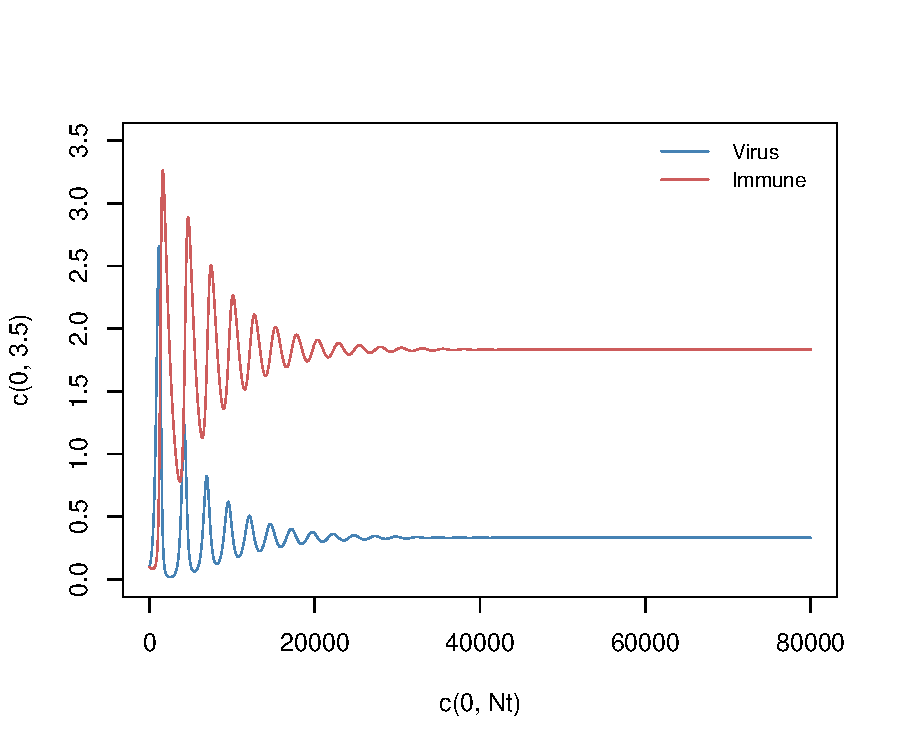
\includegraphics[width=0.5\textwidth]{inte_1}
\end{figure}

Introducendo il rumore, possiamo incorrere in alcune traiettorie negative per la carica virale. Si veda la Figura~\ref{fig:2}. Perciò ho provato due diverse strategie. La prima (a sinistra) è stata forzare la positività ribaltando il valore rispetto all'asse $x$, con la funzione modulo. La seconda (a destra) è stata diminuire il passo temporale.

\begin{figure}[ht]
\centering
\caption{A sinistra simulazione ottenuta con il Codice~\ref{lst:2}, a destra con il Codice~\ref{lst:3}.}\label{fig:2}
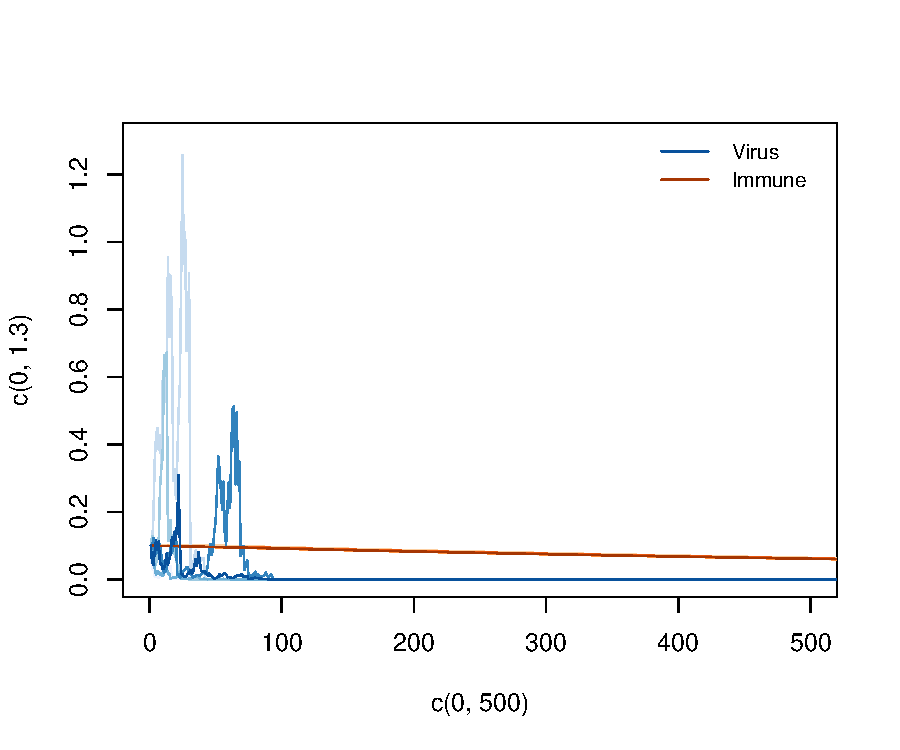
\includegraphics[width=0.49\textwidth]{inte_3}
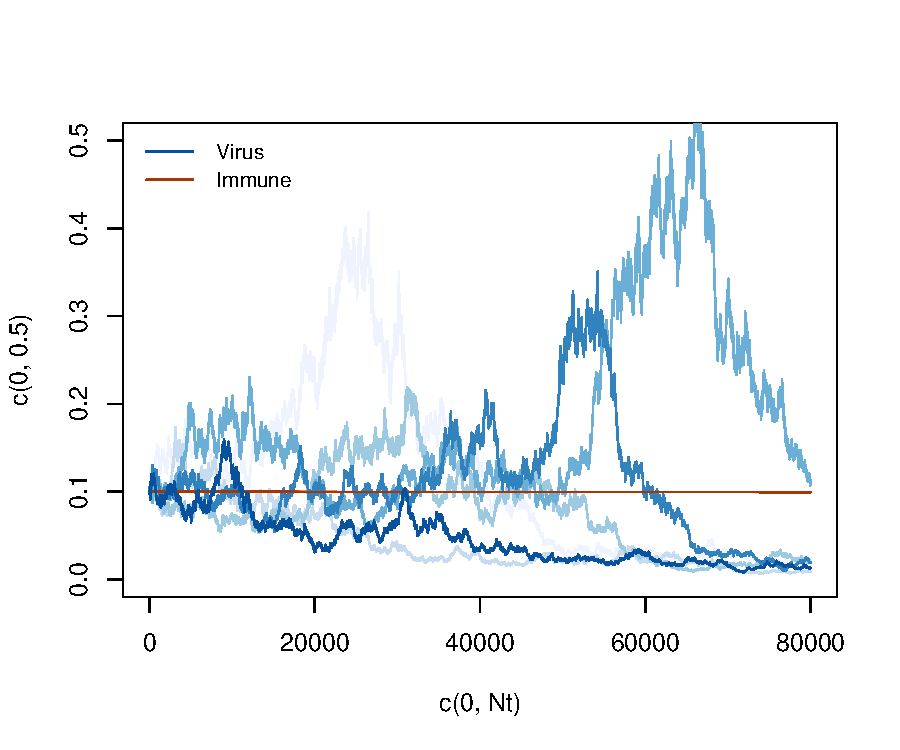
\includegraphics[width=0.49\textwidth]{inte_2}
%\emph{ricorda di includere immagini (sono pesanti, quindi le metto dopo)}
\end{figure}

In entrambi i casi osserviamo che la positività delle traiettorie viene mantenuta e che sparisce l'andamento oscillatorio dovuto all'interazione fra le due popolazioni. La risposta immunitaria si stabilizza da subito intorno al suo valore iniziale, mentre la carica virale può avere comportamenti molto diversi. Osserviamo che forzare la positività induce la carica virale a essere neutralizzata molto velocemente dal sistema immunitario. Nel secondo caso, invece, quasi tutte le traiettorie della carica virale arrivano ad annullarsi, ma sono precedute da uno o più periodi di infezione acuta. 

\section{Buona positura del sistema}
In seguito ho studiato la buona positura del sistema. Dato che il termine di diffusione è solo localmente lipschitziano, abbiamo solo localmente esistenza forte e unicità ``pathwise'' (Theorem 5, Chapter 1). Sia $X_t^{x_0}=(V_t,I_t)$ la soluzione con condizione iniziale $x_0=(v_0,i_0)\in (0,+\infty)^2$ definita per $t\in [0,T]$. 

\textbf{Step 1} (positività delle traiettorie). Proviamo che $V_t$ e $I_t$ sono strettamente positivi per ogni $t\in [0,T]$. Consideriamo il tempo d'arresto $$\tau_R := \inf \Set{t\leq T : ||X_t||_2\geq R}.$$
Mostriamo equivalentemente che per $t< \tau_0:=\inf\Set{t\leq \tau : V_t \leq 0}$ il processo $\log V_t$ è limitato da una costante dipendente solo da $R$ e perciò $\tau_0=\tau_R$. Infatti \begin{align*}
d\log V_t & = \frac{1}{V_t} dV_t -\frac{1}{2V_t^2} d[V]_t \\
&= (q-pI_t)dt + (V_{\max}-V_t)dW_t -\frac{1}{2}(V_{\max}-V_t)^2dt 
\end{align*}
che in modulo è controllato da una costante $R$-dependent per $t\leq \tau_0$. Dunque $\inf_{t\leq \tau_0}V_t$ è strettamente positivo e dunque $\tau_0=\tau_R$. Allo stesso modo, per $I_t$, se $\tau_0:=\inf\Set{t< \tau : I_t \leq 0}$ si ha che \begin{align*}
d\log I_t &= (cV_t-b)dt,
\end{align*}
che è limitato se $t\leq \tau_R$, e dunque vale lo stesso ragionamento fatto per $V_t$. Dato che $R$ è arbitrario, $X_t^{x_0}$ si mantiene nel primo quadrante per ogni $t\leq T$. 

\textbf{Step 2} (limitazione a priori). Proviamo che $V_t<V_{\max}$ per $t\in [0,T]$. Segue da un ragionamento analogo a quello dello Step 1, solo considerando il processo $Y_t=V_{\max}-V_t$. Finché $t< \tau_0=\inf \Set{t\leq \tau_R: Y_t\leq 0}$, valgono le seguenti uguaglianze: \begin{align*}
dY_t &= -(q-pI_t)V_tdt - V_t(V_{\max}-V_t)dW_t, \\
d\log Y_t &= -(q-pI_t)\frac{V_t}{V_{\max}-V_t} dt - V_tdW_t -\frac{1}{2}V_t^2dt
\end{align*}
Se $V_{\max}\geq 2$, allora finché $t\leq \tau_0$ è vero che $\left|\frac{V_t}{V_{\max}-V_t} \right|=\frac{V_t}{V_{\max}-V_t}\leq R$. Perciò per tempi $t$ con la detta limitazione, otteniamo che $\inf_{t\leq \tau_0}|\log Y_t|$ è limitato da una costante che dipende solo da $R$. Perciò $\inf_{t\leq \tau_0} {Y_t}$ è strettamente positivo e dunque $\tau_R=\tau_0$, cioè $V_t\leq V_{\max}$. Da questo ricaviamo anche una limitazione anche per $I_t$ dato che $dI_t \leq (cV_{\max}-b)dt$.

\textbf{Step 3} (strong existence e pathwise uniqueness globali). Abbiamo ottenuto che $||X_t^{x_0}||_2$ è limitata per ogni $t\in [0,T]$ e $x_0\in (0,+\infty)^2$. Possiamo perciò promuovere a globale l'esistenza locale di soluzioni forti e uniche ``pathwise''. 

\textbf{Step 4} (path-by-path existence? uniqueness?) Ha senso parlare di esistenza path-by-path? Abbiamo dato la definizione solo per coefficienti di diffusione indipendenti da $(t,x)$, così da essere sicuri che per quasi ogni $\omega$ il processo $\sqrt{Q}W_t$ avesse traiettorie continue (Definition 4, Chapter 1). Credo che nel nostro caso si possa fare altrettanto, dal momento che la limitazione su $V_t$ ci permette di concludere che l'integrale stocastico $$\int_0^t V_s(V_{\max}-V_s) dW_s$$
è una martingala: ne esiste perciò una versione continua. 


%Il primo approccio è stato studiare la norma euclidea di $X_t=(V_t,I_t)$. Con la formula di Ito ricaviamo che
%\begin{align*}
%d||X_t||_2^2 &= 2V_t dV_t + 2I_t dI_t +d[V_t] \\
%&=2V_t^2\left(q-pI_t\right)dt + V_t^2(V_{\max}-V_t)dW_t +2 I_t^2\left(cV_t-b\right)dt \\
%&\qquad + V_t^2(V_{\max}-V_t)^2dt.
%\end{align*}
%Passando al valore atteso otteniamo
%\begin{align*}\tag{2}
%\E{||X_t||_2^2} & = ||X_0||_2^2 + \E{\int_0^t 2V_s^2\left(q-pI_s\right)+2 I_s^2\left(cV_s-b\right)ds} \\
%&\qquad + \E{\int_0^t V_s^2(V_{\max}-V_s)dW_s}.
%\end{align*}
%Vorrei concludere che per un'opportuna costante $K$ vale la seguente disuguaglianza: \begin{equation}\tag{3}
%\E{||X_t||_2^2} \leq  ||X_0||_2^2 + \E{\int_0^t 2K||X_t||_2^2 ds} ,
%\end{equation}
%così da applicare Gronwall e concludere che 
%\begin{equation}
%aaa
%\end{equation}

\addcontentsline{toc}{section}{Lista dei codici}
\lstlistoflistings

\begin{lstlisting}[language=R, caption={\texttt{deterministico.R}}, label=lst:1] 
# Modello deterministico
# Parametri 
{
  N=10; Nt=80000; dt=0.009
  lam=1; d=0.1; beta=0.1; a=0.2
  p=0.3; c=0.3; b=0.1
}
# Valori iniziali
{
  S=1:Nt; I=S; CTL=S
  S[1]=5; I[1]=0.1; CTL[1]=0.1
}
# Metodo di Eulero
{
  for (t in 1:(Nt-1)){
    S[t+1] = S[t] + dt*(lam - d*S[t] - beta*S[t]*V[t])
    V[t+1] = I[t] + dt*V[t]*(beta*S[t] - a*V[t] - p*I[t]) 
    I[t+1] = I[t] + dt*I[t]*(c*V[t] - b)  
  }
}
# Plot
{
  plot(c(0,Nt),c(0,3.5), type="n")
  lines(V,col="steelblue")
  lines(I,col="indianred")
  legend("topright",legend = c("Virus","Immune"), col=c("steelblue","indianred"),lty=rep(1,2),horiz=FALSE, bty='n', cex=0.8)
}
#
\end{lstlisting}

\begin{lstlisting}[language=R, caption={\texttt{aleatorio1.R}}, label=lst:2] 
# Modello aleatorio con ribaltamento delle traiettorie negative
# Parametri
{
  Nt = 80000; dt = 0.01; Nsample = 6
  lam=1; d=0.1; beta=0.1; a=0.2; 
  p=0.3; c=0.3; b=0.1
  nat = (beta*lam*c)/(beta*b+c*d); mor = a
  sc = (lam*c)/(beta*b+c*d) # Valore di S all'equilibrio
  sigma = 1
}
# Valori iniziali
{
  V = matrix(0,Nsample,Nt)
  I = V; Vmax = 5
  V[,1] = 0.1; I[,1] = 0.1
}
# Metodo di Eulero con controllo sul numero di traiettorie negative
{
  max_rep = 1
  neq.traj = rep(0,max_rep)
  for (j in (1:max_rep)) {
    for (t in (1:(Nt-1))) {
      V[,t+1] = abs(V[,t] + dt*(nat-mor-p*I[,t])*V[,t] + V[,t]*(Vmax-V[,t])*sqrt(dt)*sigma*rnorm(Nsample))
      I[,t+1] = I[,t] + dt*I[,t]*(c*V[,t]-b) 
      }
    tmp.neg.traj = rep(0,Nsample)
    for (i in (1:Nsample)) {
      tmp.neg.traj[i] = sum(V[i,]<0)+sum(I[i,]<0)
    }
    neq.traj[j] = sum(tmp.neg.traj>0)
    }
  print('In media le traiettorie negative sono')
  print(mean(neq.traj))
}
# Plot
{
  plot(c(0,500),c(0,1.3),type="n")
  library(RColorBrewer)
  colV <- brewer.pal(Nsample, "Blues")
  colI <- brewer.pal(Nsample, "Oranges")
  legend("topright",legend = c("Virus","Immune"), col=c(colV[Nsample],colI[Nsample]),lty=rep(1,2),horiz=FALSE, bty='n', cex=0.8)
  for (i in (1:Nsample)) {
    lines(I[i,], col = colI[i])
    lines(V[i,], col = colV[i])
  }
}
#
\end{lstlisting}

\begin{lstlisting}[language=R, caption={\texttt{aleatorio2.R}}, label=lst:3] 
# Modello aleatorio con passo temporale molto piccolo
# Parametri
{
  Nt = 80000; dt = 0.000001; Nsample = 6
  lam=1; d=0.1; beta=0.1; a=0.2; 
  p=0.3; c=0.3; b=0.1
  nat = (beta*lam*c)/(beta*b+c*d); mor = a
  sc = (lam*c)/(beta*b+c*d) # Valore di S all'equilibrio
  sigma = 1
}
# Valori iniziali
{
  V = matrix(0,Nsample,Nt)
  I = V; Vmax = 5
  V[,1] = 0.1; I[,1] = 0.1
}
# Metodo di Eulero
{
  max_rep = 1
  neq.traj = rep(0,max_rep)
  for (j in (1:max_rep)) {
  # Metodo di Eulero
    for (t in (1:(Nt-1))) {
      V[,t+1] = V[,t] + dt*(nat-mor-p*I[,t])*V[,t] + V[,t]*(Vmax-V[,t])*sqrt(dt)*sigma*rnorm(Nsample)
      I[,t+1] = I[,t] + dt*I[,t]*(c*V[,t]-b) 
      }
    tmp.neg.traj = rep(0,Nsample)
    for (i in (1:Nsample)) {
      tmp.neg.traj[i] = sum(V[i,]<0)+sum(I[i,]<0)
    }
    neq.traj[j] = sum(tmp.neg.traj>0)
    }
  print('In media le traiettorie negative sono')
  print(mean(neq.traj))
}
# Plot
{
  plot(c(0,Nt),c(0,0.5),type="n")
  library(RColorBrewer)
  colV <- brewer.pal(Nsample, "Blues")
  colI <- brewer.pal(Nsample, "Oranges")
  legend("topright",legend = c("Virus","Immune"), col=c(colV[Nsample],colI[Nsample]),lty=rep(1,2),horiz=FALSE, bty='n', cex=0.8)
  for (i in (1:Nsample)) {
    lines(I[i,], col = colI[i])
    lines(V[i,], col = colV[i])
  }
}
#
\end{lstlisting}

\end{document}
